\chapter{\label{ch:5}Nucleotide regulation of Kir6.2} 

\graphicspath{{figures/ch5/}}

\minitoc

\section{Introduction}

There are variety of ways in which mutations in Kir6.2 can lead to altered K\ATP{} channel function, and often lead to diseases of insulin secretion \cite{ashcroft_katp_2013, aguilar-bryan_neonatal_2008, hattersley_activating_2005, ashcroft_neonatal_2017, flanagan_update_2009, ashcroft_diabetes_2012, pipatpolkai_new_2020-1}.
These can be divided into two broad categories; mutations which have a ligand-independent effect, and those which affect the ligand-dependent regulation of the channel, covered in more detail in Chapter \ref{ch1-intro}.
Nucleotide inhibition of the K\ATP{} channel can be altered by mutations through three separate mechanistic routes.
A mutation which reduces sensitivity of the channel to nucleotide inhibition may act by either reducing the affinity of binding of nucleotides to Kir6.2, increasing the open probability of the channel, reducing the transduction of nucleotide binding to channel closure, or a combinatuon of all three.

Interrogation of residues in this second category is very difficult using electrophysiological measures alone, as without measuring binding of nucleotides directly it is hard to truly separate effects on open probability from effects on binding and transduction \cite{colquhoun_binding_1998}.
In this chapter, we aim to clarify the role of several residues implicated in regulating the inhibitory effect of nucleotides on K\ATP{} channel function by measuring TNP-ATP binding directly to the inhibitory nucleotide binding site on Kir6.2, where possible in conjunction with simultaneous current measurements.

\section{Nucleotide binding}

\subsection{G334D abolishes nucleotide binding}

Residue G334 of Kir6.2 is located in the C-terminal region (Figure \ref{ch5fig:g334d_loc}) and has been hypothesised to form part of the ATP binding site since electrophysiological studies demonstrated a dramatic reduction in nucleotide sensitivity upon mutation of the residue \cite{drain_katp_1998, li_open_2002, li_ligand-dependent_2005}.
In addition, mutation of this residue to aspartic acid (G334D) results in severe permanent neonatal diabetes mellitus \cite{masia_atp-binding_2007-1}.
This hypothesis was confirmed by the solving of cryo-EM structures of K\ATP{} in the presence of ATP, which revealed the close proximity of residue G334 to the bound ATP \cite{lee_molecular_2017, martin_anti-diabetic_2017, li_structure_2017, puljung_cryo-electron_2018-1}.
Mutating G334 to a total of 13 different amino acid substitutions led to a increase in the IC\textsubscript{50} for ATP by over an order of magnitude in excised patches \cite{li_ligand-dependent_2005}.
However, only two of those substitutions (R and K) resulted in any changes in nucleotide-independent channel gating when examined at the single-channel level, with unliganded $P_O$ remaining constant.
It has therefore been suggested that while G334 forms part of the ATP binding site of Kir6.2, it does not participate in channel gating or transduction of ligand binding to the channel pore.

\begin{figure}[h]
	\centering
	\begin{subfigure}[t]{0.45\textwidth}
		\caption{}\label{ch5fig:g334d_loc}
		\centering
		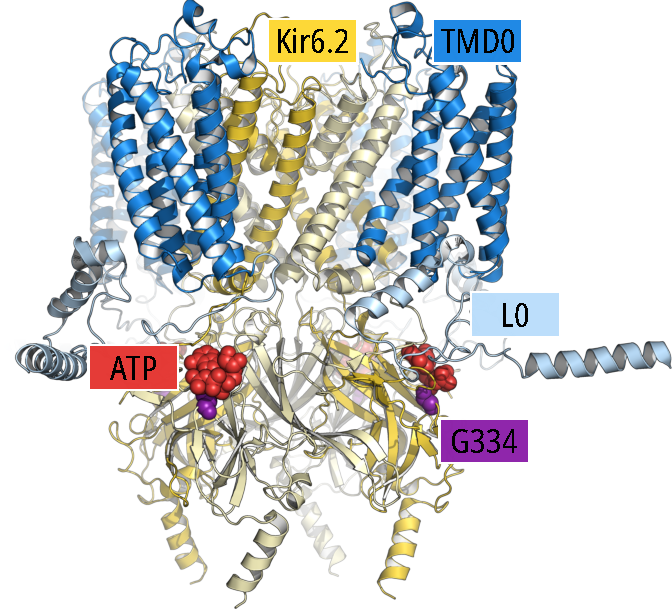
\includegraphics[width=\textwidth]{g334d_1.pdf}
	\end{subfigure}
	\hfill
	\begin{subfigure}[t]{0.45\textwidth}
		\caption{}\label{ch5fig:g334d_popfits}
		\centering
		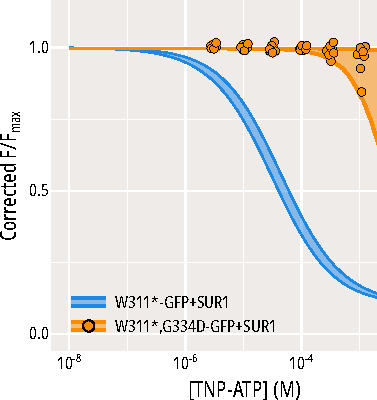
\includegraphics[width=\textwidth]{g334d_2.pdf}
	\end{subfigure}
	\vfill
	\begin{subfigure}[t]{0.9\textwidth}
		\caption{}\label{ch5fig:g334d_indfits}
		\centering
		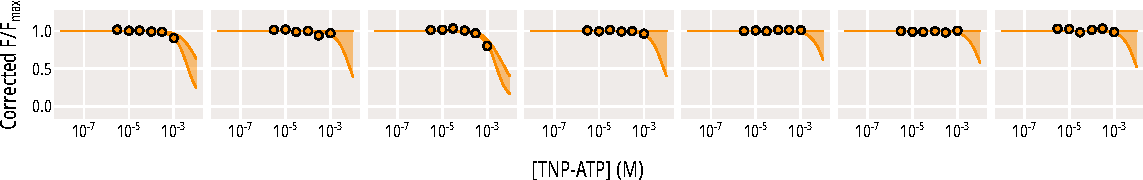
\includegraphics[width=\textwidth]{g334d_3.pdf}
	\end{subfigure}
	\vfill
	\begin{subfigure}[t]{0.7\textwidth}
		\caption{}\label{ch5fig:g334d_params}
		\centering
		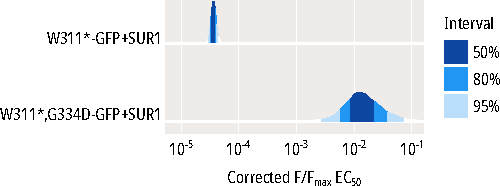
\includegraphics[width=\textwidth]{g334d_4.pdf}
	\end{subfigure}
	\caption[G334D abolishes nucleotide binding at Kir6.2]{
	\subref{ch5fig:g334d_loc} Residue G334 is shown in purple in the cryo-EM structure of K\ATP{} (PDB \#6C3P).
	Adjacent subunits of Kir6.2 are shown in two different shades of yellow, TMD0 and L0 of SUR1 are shown in two different shades of blue.
	The core of SUR1 is not shown.
	Bound ATP is shown in red.
	\subref{ch5fig:g334d_popfits} Fluorescence quenching of W311*,G334D-GFP+SUR1 by TNP-ATP in unroofed membrane patches.
	Each point represents an individual experiment.
	The smooth filled curves are the \SI{95}{\percent} intervals of the posterior probability distribution of fits to equation \ref{eq:hill} as described in the methods.
	\subref{ch5fig:g334d_indfits} Data from each experiment is shown separately.
	The smooth filled curves are the \SI{95}{\percent} intervals of the posterior predictions for each experiment.
	\subref{ch5fig:g334d_params} Posterior probability distributions for the estimated population $EC_{50}$ values are shown coloured according to their intervals.
	}\label{ch5fig:g334d}
\end{figure}

We sought to test this directly by measuring the binding of TNP-ATP in unroofed membranes to W311*,G334D-GFP+SUR1.
Fluorescence spectra captured from unroofed membrane patches expressing W311*,G334D-GFP+SUR1 were indistinguishable from those expressing W311*-GFP+SUR1.
The location of the ANAP peak and the bleaching characteristics were also identical.
We found that ANAP fluorescence from W311*,G334D-GFP+SUR1 was barely quenched by even \SI{1}{\milli\Molar} TNP-ATP (Figure \ref{ch5fig:g334d_popfits}, \ref{ch5fig:g334d_indfits}), reducing the apparant binding EC\textsubscript{50} from \SIrange{30}{45}{\micro\Molar} to at least \SI{2.8}{\milli\Molar} (Figure \ref{ch5fig:g334d_params}).
We cannot be sure of the upper bound of the apparent binding EC\textsubscript{50} given how little quenching we were able to achieve even with \SI{1}{\milli\Molar} TNP-ATP.
Unfortunately, we were unable to resolve macroscopic currents from W311*,G334D-GFP+SUR1 in excised patches despite seeing fluorescence in unroofed membranes.
Thus, we were unable to measure nucleotide inhibition of this construct ourselves.
In electrophysiological experiments on K\ATP{} channels containing the G334D mutation, other studies have found that currents are insensitive to inhibition by ATP even up to \SI{10}{\Molar} \cite{drain_katp_1998, masia_atp-binding_2007-1}.
In the framework of our MWC model, the only explanation for a dramatic decrease in both nucleotide binding and inhibition is a decrease in $K_A$, the microscopic binding affinity.
However, as we were unable to measure TNP-ATP inhibition ourselves, we were unable to determine whether the G334D substitution affected transduction in addition to this binding effect.

\section{Channel gating}

\subsection{C166S alters inhibition without affecting binding}

Residue C166 of Kir6.2 is located at the cytosolic end of the second transmembrane domain (Figure \ref{ch5fig:c166s_loc}, \cite{lee_molecular_2017, martin_anti-diabetic_2017, li_structure_2017, puljung_cryo-electron_2018-1}), and has been suggested to play a role in regulating the intrinsic gating of the channel \cite{gloyn_kcnj11_2006, trapp_molecular_1998, ribalet_atp-sensitive_2006, yang_palmitoylation_2020, loussouarn_structure_2000, enkvetchakul_kinetic_2000}.
Mutations at this residue lead to dramatically increased unliganded $P_O$ in single-channel experiments \cite{trapp_molecular_1998, enkvetchakul_kinetic_2000, ribalet_atp-sensitive_2006}, and a reduction in sensitivity to nucleotide inhibition at both single-channel and the macroscopic level \cite{trapp_molecular_1998, enkvetchakul_kinetic_2000, ribalet_atp-sensitive_2006, li_decomposition_2013, yang_palmitoylation_2020}.
In addition, two substitutions at this residue (F and Y) have been found to cause severe neonatal diabetes \cite{gloyn_kcnj11_2006}.
Electrophysiological measurements alone are not sufficient to distinguish between the reduction in sensitivity to nucleotide inhibition being caused by the increase in intrinsic $P_O$ alone, or whether there is an additional disregulation of transduction.

We measured TNP-ATP binding to W311*,C166S-GFP+SUR1 in unroofed membranes to determine the how mutations at C166 reduce sensitivity to nucleotide inhibition (Figure \ref{ch5fig:c166s_unroofed}).
We observed no real change in binding of TNP-ATP to the channel, with an EC\textsubscript{50} of \SIrange{44}{74}{\micro\Molar}.
If the C166S mutation solely increases the $P_O$ of the channel, we would expect an increase in the apparent EC\textsubscript{50} of nucleotide binding due to the preference of nucleotides for the closed state of the channel.
This finding therefore suggests a role for C166 in the transduction of nucleotide binding to the channel pore.

\begin{figure}[h]
	\centering
	\begin{subfigure}[t]{0.45\textwidth}
		\caption{}\label{ch5fig:c166s_loc}
		\centering
		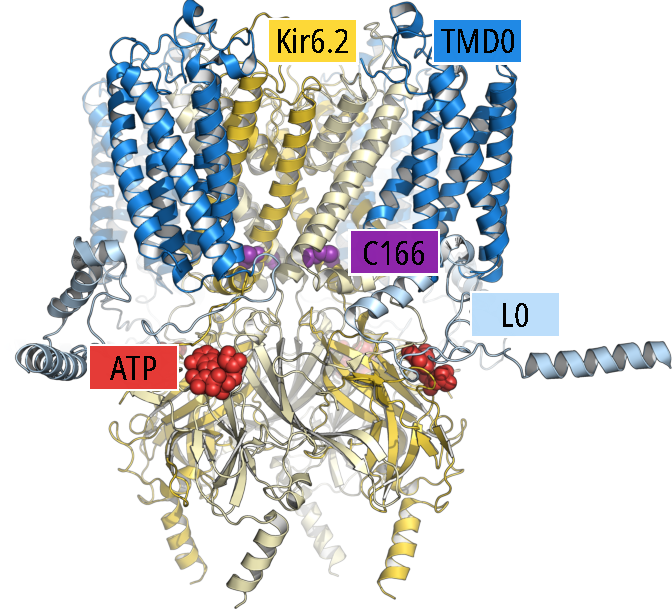
\includegraphics[width=\textwidth]{c166s_1.pdf}
	\end{subfigure}
	\hfill
	\begin{subfigure}[t]{0.45\textwidth}
		\caption{}\label{ch5fig:c166s_popfits}
		\centering
		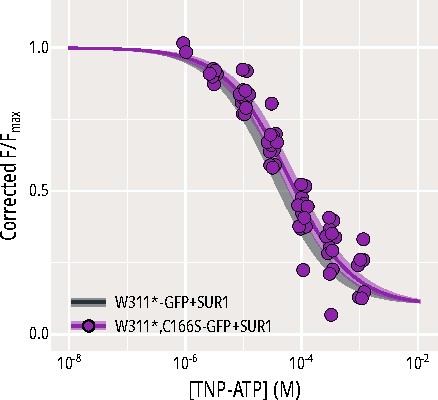
\includegraphics[width=\textwidth]{c166s_2.pdf}
	\end{subfigure}
	\vfill
	\begin{subfigure}[t]{0.9\textwidth}
		\caption{}\label{ch5fig:c166s_indfits}
		\centering
		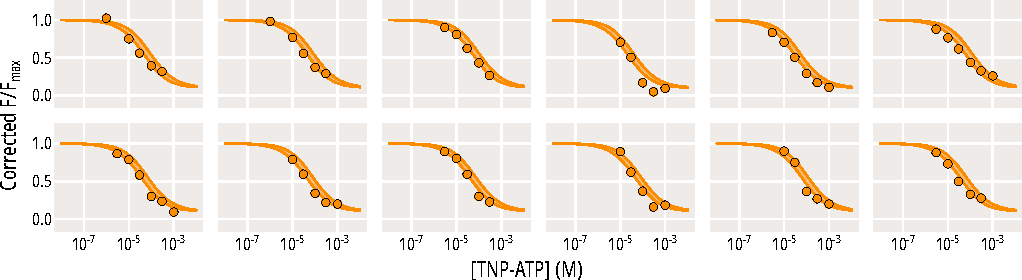
\includegraphics[width=\textwidth]{c166s_3.pdf}
	\end{subfigure}
	\vfill
	\begin{subfigure}[t]{0.7\textwidth}
		\caption{}\label{ch5fig:c166s_params}
		\centering
		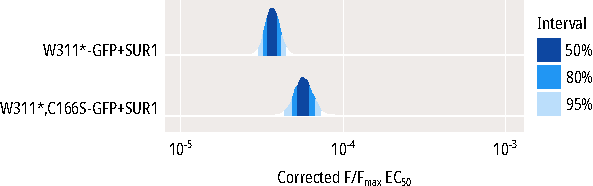
\includegraphics[width=\textwidth]{c166s_4.pdf}
	\end{subfigure}
	\caption[C166S does not alter nucleotide binding]{
	\subref{ch5fig:c166s_loc} Residue C166 is shown in purple in the cryo-EM structure of K\ATP{} (PDB \#6C3P).
	Adjacent subunits of Kir6.2 are shown in two different shades of yellow, TMD0 and L0 of SUR1 are shown in two different shades of blue.
	The core of SUR1 is not shown.
	Bound ATP is shown in red.
	\subref{ch5fig:c166s_popfits} Fluorescence quenching of W311*,C166S-GFP+SUR1 by TNP-ATP in unroofed membrane patches.
	Each point represents an individual experiment.
	The smooth filled curves are the \SI{95}{\percent} intervals of the posterior probability distribution of fits to equation \ref{eq:hill} as described in the methods.
	\subref{ch5fig:c166s_indfits} Data from each experiment is shown separately.
	The smooth filled curves are the \SI{95}{\percent} intervals of the posterior predictions for each experiment.
	\subref{ch5fig:c166s_params} Posterior probability distributions for the estimated population $EC_{50}$ values are shown coloured according to their intervals.
	}\label{ch5fig:c166s_1}
\end{figure}

To investigate this further, we excised patches expressing W311*,C166S-GFP+SUR1 and measured current inhibition and fluorescence quenching by TNP-ATP simultaneously (Figure \ref{ch5fig:c166s_traces}).
We found that the apprent affinity for nucleotide binding was indistinguishable from that for W311*-GFP+SUR1, and similar to our observations in unroofed membranes (Figure \ref{ch5fig:c166s_popfits_2}, EC\textsubscript{50} of \SIrange{26}{218}{\micro\Molar}).
Consistent with the literature, we did observe a large reduction in the apparent sensitivity of W311*,C166S-GFP+SUR1 currents to inhibition by TNP-ATP (Figure \ref{ch5fig:c166s_popfits_3}, IC\textsubscript{50} of at least \SI{155}{\micro\Molar}).
Intuitively, a change in nucleotide-dependent channel gating which is not accompanied by a change in nucleotide binding must be due (at least in part) to a change in the transduction of nucleotide binding to channel gating.

\begin{figure}[h]
	\centering
	\begin{subfigure}[t]{0.6\textwidth}
		\caption{}\label{ch5fig:c166s_traces}
		\centering
		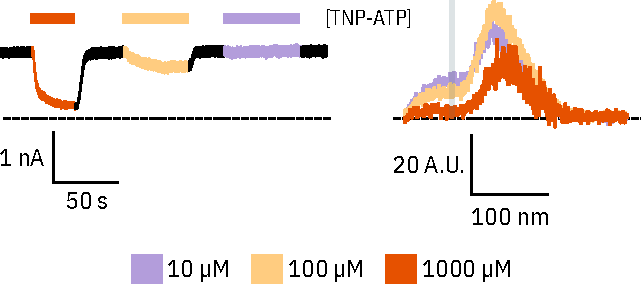
\includegraphics[width=\textwidth]{c166s_5.pdf}
	\end{subfigure}
	\hfill
	\begin{subfigure}[t]{0.3\textwidth}
		\caption{}\label{ch5fig:c166s_popfits_2}
		\centering
		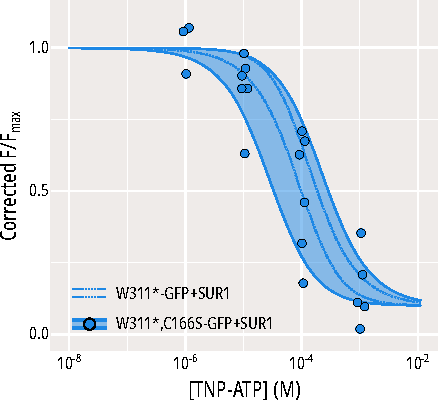
\includegraphics[width=\textwidth]{c166s_6.pdf}
	\end{subfigure}
	\vfill
	\begin{subfigure}[t]{0.3\textwidth}
		\caption{}\label{ch5fig:c166s_popfits_3}
		\centering
		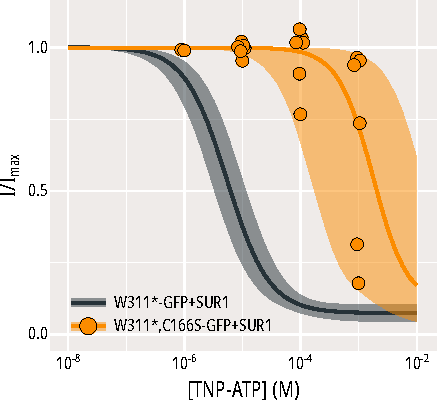
\includegraphics[width=\textwidth]{c166s_7.pdf}
	\end{subfigure}
	\hfill
	\begin{subfigure}[t]{0.6\textwidth}
		\caption{}\label{ch5fig:c166s_params_2}
		\centering
		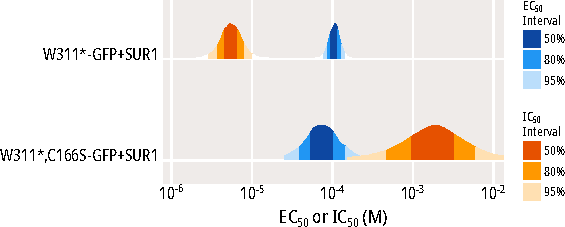
\includegraphics[width=\textwidth]{c166s_8.pdf}
	\end{subfigure}
	\vfill
	\begin{subfigure}[t]{0.9\textwidth}
		\caption{}\label{ch5fig:c166s_indfits_2}
		\centering
		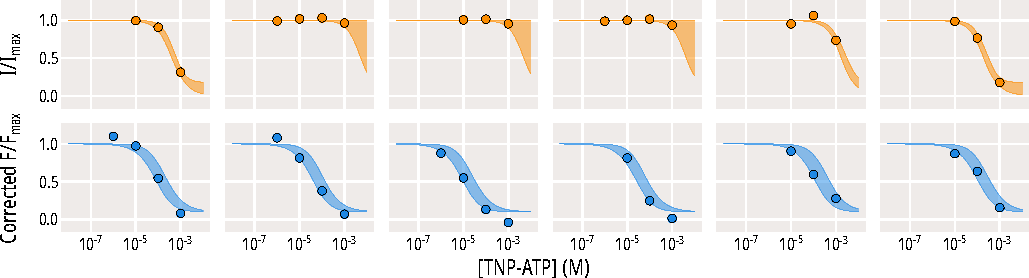
\includegraphics[width=\textwidth]{c166s_9.pdf}
	\end{subfigure}
	\caption[C166S alters sensitivity to nucleotide inhibition]{
	\subref{ch5fig:c166s_traces} Current inhibition (left) and fluorescence quenching (right) from an excised patch expressing W311*,C166S-GFP+SUR1.
	The concentration of TNP-ATP perfused is shown by colour.
	The location of the peak ANAP fluorescence is marked as a grey box.
	\subref{ch5fig:c166s_popfits_2} Fluorescence quenching of W311*,C166S-GFP+SUR1 by TNP-ATP in excised patches.
	Each point represents an individual experiment.
	The smooth filled curves are the \SI{95}{\percent} intervals of the posterior probability distribution of fits to equation \ref{eq:hill} as described in the methods.
	\subref{ch5fig:c166s_popfits_3} Current inhibition of W311*,C166S-GFP+SUR1 by TNP-ATP in excised patches.
	Each point represents an individual experiment.
	The smooth filled curves are the \SI{95}{\percent} intervals of the posterior probability distribution of fits to equation \ref{eq:hill} as described in the methods.
	\subref{ch5fig:c166s_params_2} Posterior probability distributions for the estimated population EC\textsubscript{50} (blue) and IC\textsubscript{50} (orange) values are shown shaded according to their intervals.
	\subref{ch5fig:c166s_indfits_2} Data from each experiment is shown separately; each column represents one excised patch..
	The smooth filled curves are the \SI{95}{\percent} intervals of the posterior predictions for each experiment.
	}\label{ch5fig:c166s_2}
\end{figure}

Fitting our data to the MWC-type model described previously (Figure \ref{ch5fig:c166s_mwc_fit_1}, \ref{ch5fig:c166s_mwc_fit_2}), we found that in addition to the effects of the C166S mutation on the intrinsic open probability of K\ATP{}, there is a striking shift in $D_A$ (Figure \ref{ch5fig:c166s_mwc_params_1}).
This shift to a value much closer to unity indicates that binding of TNP-ATP to W311*,C166S-GFP+SUR1 favours the closed state far less than binding of TNP-ATP to W311*-GFP+SUR1.
Equivalently, binding of TNP-ATP to the mutant channel is less able to induce closure of the pore.
Thus, even at millimolar concentrations of TNP-ATP when all of the Kir6.2 subunits are predicted to be bound by nucleotide, the mutant K\ATP{} channels are still able to open.

\begin{figure}[h]
	\centering
	\begin{subfigure}[t]{0.45\textwidth}
		\caption{}\label{ch5fig:c166s_mwc_fit_1}
		\centering
		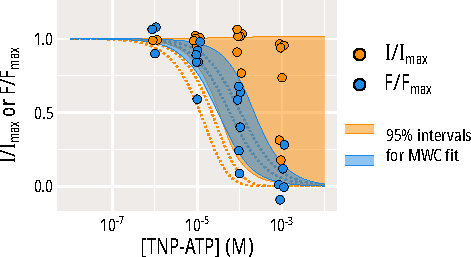
\includegraphics[width=\textwidth]{mwc_c166s_1.pdf}
	\end{subfigure}
	\hfill
	\begin{subfigure}[t]{0.45\textwidth}
		\caption{}\label{ch5fig:c166s_mwc_fit_2}
		\centering
		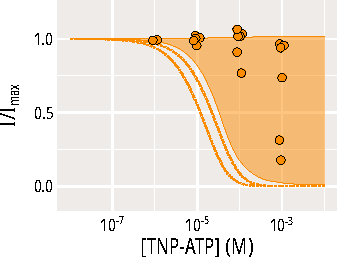
\includegraphics[width=\textwidth]{mwc_c166s_3.pdf}
	\end{subfigure}
	\vfill
	\begin{subfigure}[t]{0.9\textwidth}
		\caption{}\label{ch5fig:c166s_mwc_params_1}
		\centering
		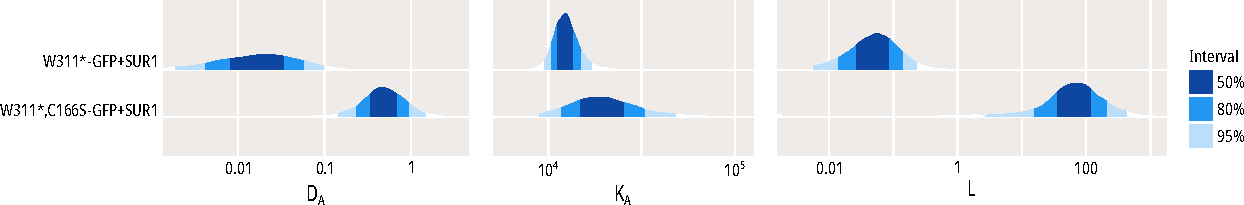
\includegraphics[width=\textwidth]{mwc_c166s_2.pdf}
	\end{subfigure}
	\caption[C166S alters transduction of nucleotide binding to Kir6.2]{
	\subref{ch5fig:c166s_mwc_fit_1}, \subref{ch5fig:c166s_mwc_fit_2} Nucleotide binding (\subref{ch5fig:c166s_mwc_fit_1}) and current inhibition (\subref{ch5fig:c166s_mwc_fit_2}) of W311*,C166S-GFP+SUR1 by TNP-ATP in excised patches, data the same as in Figure \subref{ch5fig:c166s_popfits_2}, \subref{ch5fig:c166s_popfits_3}.
	The solid lines are the \SI{95}{\percent} intervals of the posterior probability distribution of fits to the MWC model paramaterised in equations \ref{eq:mwc_binding} and \ref{eq:normalised_po}.
	The dotted lines are the equivalent intervals for MWC fits to the W311*-GFP+SUR1 construct as shown in Figure \ref{ch3fig:pcf_1}.
	White circles are the inhibition of current by \SI{10}{\milli\Molar} ATP in separate experiments.
	\subref{ch5fig:c166s_mwc_params_1} Posterior probability distributions for the estimated population $L$, $D_A$ and $K_A$ values are shown shaded according to their intervals.
	}\label{ch5fig:c166s_3}
\end{figure}

Notably, the MWC fit to the current inhibition data has wide \SI{95}{\percent} posterior probability intervals (Figure \ref{ch5fig:c166s_mwc_fit_2}).
Unfortunately, we were not able to use higher concentrations of TNP-ATP due to its purification as a TEA\textsuperscript{+} salt.
High \si{\milli\Molar} concentrations of TEA\textsuperscript{+} inhibit K\ATP{} channels, and we determined that for W311*-GFP+SUR1 and W311*,C166S-GFP+SUR1 concentrations of above \SI{1}{\milli\Molar} TEA\textsuperscript{+} began to inhibit currents to an extent that would interfere with our measurements (Figure \ref{ch5fig:tea_trace}, \ref{ch5fig:tea_drc}).
The precise ratio of TEA\textsuperscript{+} to TNP-ATP in our solutions is unknown, but is assumed to be between 1:1 and 3:1.
Any additional inhibition observed at TNP-ATP concentrations greater than \SI{1}{\milli\Molar} for W311*,C166S-GFP+SUR1 will therefore be (at least in part) due to the presence of TEA\textsuperscript{+}.
However, we do see that even at concentrations of \SI{10}{\milli\Molar} ATP, W311*,C166S-GFP+SUR1 is not fully inhibited (Figure \ref{ch5fig:c166s_mwc_fit_2}, open circle).

Curiously, despite the wide posterior probability intervals for the MWC fit to the observed current inhibiton data in Figure \ref{ch5fig:c166s_mwc_fit_2}, the probability distributions for the underlying parameter values for W311*,C166S-GFP+SUR1 are not much wider than those observed for W311*-GFP+SUR1 (Figure \ref{ch5fig:c166s_mwc_params_1}).
Thus, the variability of current inhibition observed for \SI{1}{\milli\Molar} TNP-ATP is not due to increased uncertainty in our MWC parameter estimates.
Instead, the variability may reflect that the C166S substitution alters the nucleotide regulation of the K\ATP{} channel such that small changes in the energetics of the underlying gating mechanism result in large changes in the observed current.
This may help to explain the differences in inhibition of K\ATP{} channels with substitutions at C166 by high nucleotide concentrations observed across multiple electrophysiological studies \cite{trapp_mechanism_1998, enkvetchakul_atp_2001-1, ribalet_atp-sensitive_2006-1, yang_palmitoylation_2020}.

\begin{figure}[h]
	\centering
	\begin{subfigure}[t]{0.45\textwidth}
		\caption{}\label{ch5fig:tea_trace}
		\centering
		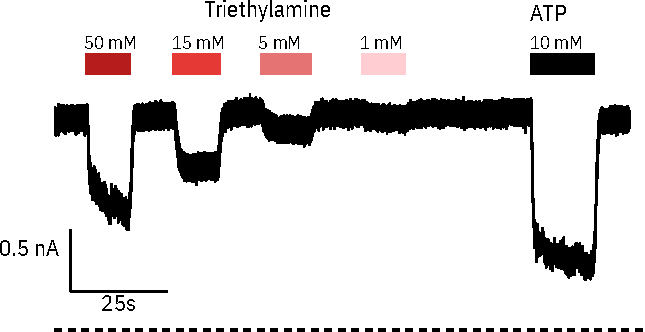
\includegraphics[width=\textwidth]{tea_trace.pdf}
	\end{subfigure}
	\hfill
	\begin{subfigure}[t]{0.45\textwidth}
		\caption{}\label{ch5fig:tea_drc}
		\centering
		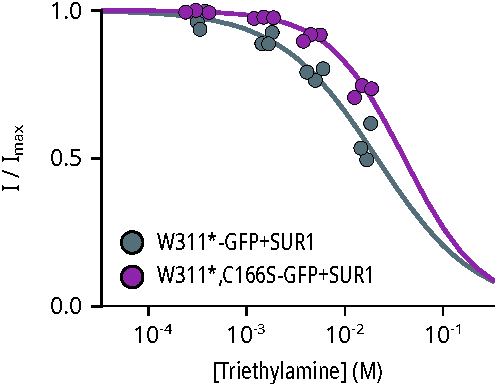
\includegraphics[width=\textwidth]{tea_drc.pdf}
	\end{subfigure}
	\caption[TEA\textsubscript{+} inhibits K\ATP{} channels at high concentrations]{
	\subref{ch5fig:tea_trace} Representative current trace from an excised patch expressing W311*,C166S-GFP+SUR1.
	Applications of different concentrations of TEA\textsubscript{+} are indicated by bars shaded red, and application of \SI{10}{\milli\Molar} ATP is indicated in black.
	The zero-current level is marked with a dotted line.
	\subref{ch5fig:tea_drc} Concentration-response data for W311*-GFP+SUR1 (blue) and W311*,C166S-GFP+SUR1 (green) current inhibition by TEA\textsubscript{+}.
	The lines are fits to equation \ref{eq:hill} with $I_{max}$ fixed to 0.
	}\label{ch5fig:c166s_4}
\end{figure}

\subsection{Mutations at E179 alter both inhibition and binding}

Residue E179 of Kir6.2 is located in the C-terminal region of Kir6.2 between the inhibitory nucleotide binding site and the proposed PIP\textsubscript{2} binding site.
In one early predicted structures of Kir6.2, it was theorised that E179 would form part of the nucleotide binding pocket directly, potentially coordinating the adenine ring of ATP directly through hydrogen bonding \cite{antcliff_functional_2005}.
In another, it was hypothesised to form part of the PIP\textsubscript{2} binding pocket instead \cite{haider_identification_2007}.
Electrophysiological experiments painted a confusing picture of the residues role \cite{antcliff_functional_2005}.
Mutation to an amino acid capable of forming hydrogen bonds (Q) resulted in no change in the IC\textsubscript{50} for nucleotide inhibition (although a separate study found that Q increased the IC\textsubscript{50} \cite{proks_involvement_1999}), while only one of two amino acids incapable of forming hydrogen bonds tested (M and L) resulted in an increased IC\textsubscript{50}.
In addition, mutation of the residue to asparagine (which is not capable of forming hydrogen bonds) not only dramatically increased the nucleotide IC\textsubscript{50}, but increased the intrinsic open probability of the channel \cite{antcliff_functional_2005}.

\begin{figure}[h]
	\centering
	\begin{subfigure}[t]{0.45\textwidth}
		\caption{}\label{ch5fig:e179_loc}
		\centering
		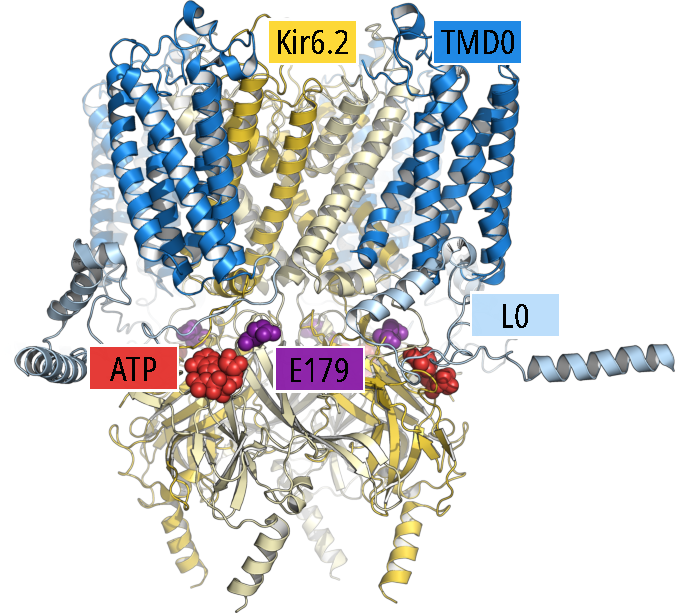
\includegraphics[width=\textwidth]{e179_1.pdf}
	\end{subfigure}
	\hfill
	\begin{subfigure}[t]{0.45\textwidth}
		\caption{}\label{ch5fig:e179_atp_popfits}
		\centering
		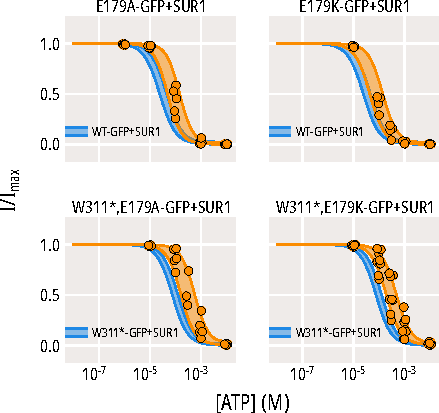
\includegraphics[width=\textwidth]{e179_2.pdf}
	\end{subfigure}
	\vfill
	\begin{subfigure}[t]{0.45\textwidth}
		\caption{}\label{ch5fig:e179_tnpatp_popfits_1}
		\centering
		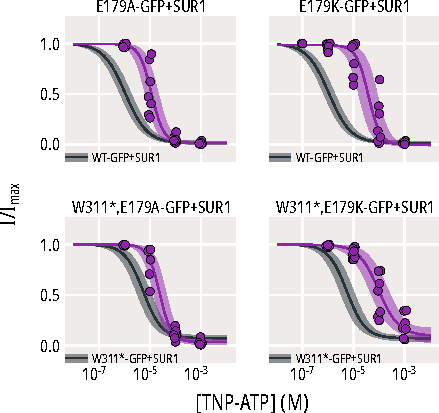
\includegraphics[width=\textwidth]{e179_3.pdf}
	\end{subfigure}
	\hfill
	\begin{subfigure}[t]{0.45\textwidth}
		\caption{}\label{ch5fig:e179_tnpatp_popfits_2}
		\centering
		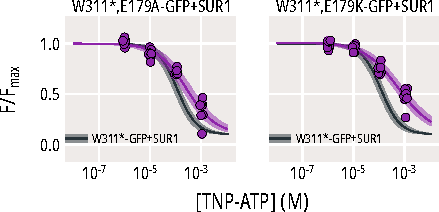
\includegraphics[width=\textwidth]{e179_4.pdf}
	\end{subfigure}
	\caption[Functional effects of E179 mutations]{
	\subref{ch5fig:e179_loc} Residue E179 is shown in purple in the cryo-EM structure of K\ATP{} (PDB \#6C3P).
	Adjacent subunits of Kir6.2 are shown in two different shades of yellow, TMD0 and L0 of SUR1 are shown in two different shades of blue.
	The core of SUR1 is not shown.
	Bound ATP is shown in red.
	\subref{ch5fig:e179_atp_popfits}, \subref{ch5fig:e179_tnpatp_popfits_1} Current inhibition of E179 mutants in the WT-GFP+SUR1 and W311*-GFP+SUR1 background by ATP (\subref{ch5fig:e179_atp_popfits}) or TNP-ATP (\subref{ch5fig:e179_tnpatp_popfits_1}).
	Each point represents an individual experiment.
	The smooth filled curves are the \SI{95}{\percent} intervals of the posterior probability distribution of fits to equation \ref{eq:hill} as described in the methods.
	\subref{ch5fig:e179_tnpatp_popfits_2} Fluorescence quenching of E179 mutants in the W311*-GFP+SUR1 background by TNP-ATP acquired simultaneously with the inhibition data in panel \subref{ch5fig:e179_tnpatp_popfits_1}.
	Each point represents an individual experiment.
	The smooth filled curves are the \SI{95}{\percent} intervals of the posterior probability distribution of fits to equation \ref{eq:hill} as described in the methods.
	\subref{ch5fig:e179_ec50_fits} Posterior probability distributions for the estimated population $IC_{50}$ or $EC_{50}$ values are shown in purple ($IC_{50}$ for ATP inhibition), orange ($IC_{50}$ for TNP-ATP inhibition), or blue ($EC_{50}$ for TNP-ATP binding).
	Each distribution is shaded with respect to its intervals.
	}\label{ch5fig:e179_1}
\end{figure}

\begin{figure}[h]
	\centering
	\begin{subfigure}[t]{0.9\textwidth}
		\caption{}\label{ch5fig:e179_ec50_fits}
		\centering
		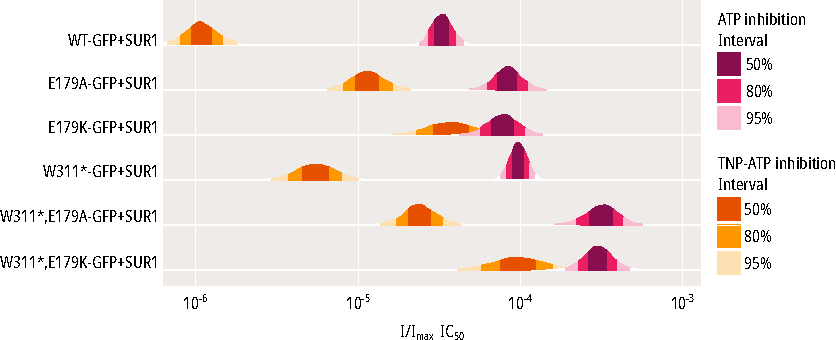
\includegraphics[width=\textwidth]{e179_5.pdf}
	\end{subfigure}
	\caption[E179 mutations $EC_{50}$ parameters]{
	\subref{ch5fig:e179_ec50_fits} Posterior probability distributions for the estimated population $IC_{50}$ or $EC_{50}$ values are shown in purple ($IC_{50}$ for ATP inhibition), orange ($IC_{50}$ for TNP-ATP inhibition), or blue ($EC_{50}$ for TNP-ATP binding).
	Each distribution is shaded with respect to its intervals.
	}\label{ch5fig:e179_1a}
\end{figure}

The cryo-EM structures of K\ATP{} in complex with ATP revealed that bound ATP adopted a radically different conformation to that proposed in early models, and the E179 side chain actually lies over \SI{8}{\angstrom} away from bound ATP \cite{lee_molecular_2017, martin_anti-diabetic_2017, li_structure_2017, puljung_cryo-electron_2018-1} (FIgure \ref{ch5fig:e179_loc}.
Unfortunately, no structure has been resolved in the presence of PIP\textsubscript{2} to date.
However, coarse-grained molecular dynamics simulations using the cryo-EM structures as a starting point indicate that E179 may form part of the PIP\textsubscript{2} binding pocket \cite{pipatpolkai_evaluating_2020}.
In addition, mutation to E179K results in reduced inhibition of the channel by the sequestering agent neomycin - potentially due to an increased affinity of the mutated residue for PIP\textsubscript{2} \cite{pipatpolkai_evaluating_2020}.

To attempt to resolve the precise role of E179 in nucleotide binding and inhibition, we first determined how ATP and TNP-ATP inhibiton of K\ATP{} channels was affected by mutation of E179 to A or K (Figure \ref{ch5fig:e179_atp_popfits}, \ref{ch5fig:e179_tnpatp_popfits_1}.
For E179A-GFP+SUR1 and E179K-GFP+SUR1, we observed an increase in IC\textsubscript{50} for both ATP and TNP-ATP inhibition (Figure \ref{ch5fig:e179_ec50_fits}).
ATP inhibition did not seem to be influenced by the identity of the replacement amino acid (\SIrange{49}{145}{\micro\Molar} and \SIrange{43}{138}{\micro\Molar} respectively), while TNP-ATP inhibition was less reduced by mutation to an A than a K (\SIrange{6.5}{21}{\micro\Molar} and \SIrange{16}{87}{\micro\Molar} respectively).
Introducing the mutations into the ANAP-labelled construct did not affect the relative changes in inhibition by either nucleotide, with ATP inhibition occurring at similar IC\textsubscript{50}s for A and K (\SIrange{162}{562}{\micro\Molar} and \SIrange{191}{479}{\micro\Molar} respectively) and with A increasing the IC\textsubscript{50} for TNP-ATP less than K (\SIrange{14}{44}{\micro\Molar} and \SIrange{42}{224}{\micro\Molar} respectively).
Measurements of TNP-ATP binding mirrored our observations for current inhibition by TNP-ATP, with mutation to both A and K resulting in an increased apparant binding EC\textsubscript{50}, with A having less of an effect than K (\SIrange{166}{417}{\micro\Molar} and \SIrange{347}{813}{\micro\Molar} respectively).
Fitting the combined data to the MWC-type model, we found that both mutations resulted in a decreased $K_A$ estimate, with no apparent change in $L$.
In addition, mutation to a K led to a $D_A$ value closer to unity than for E or the wild-type A (Figure \ref{ch5fig:e179_2}).

\begin{figure}[h]
	\centering
	\begin{subfigure}[t]{0.9\textwidth}
		\caption{}\label{ch5fig:mwc_e179_1}
		\centering
		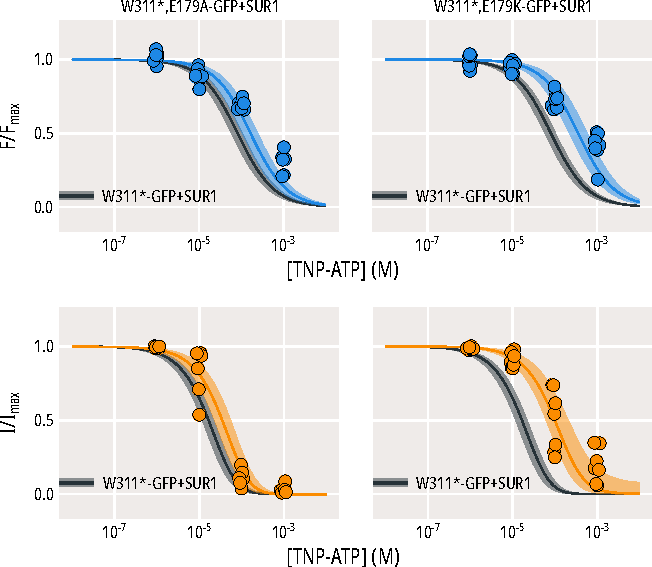
\includegraphics[width=\textwidth]{mwc_e179_1.pdf}
	\end{subfigure}
	\vfill
	\begin{subfigure}[t]{0.9\textwidth}
		\caption{}\label{ch5fig:mwc_e179_2}
		\centering
		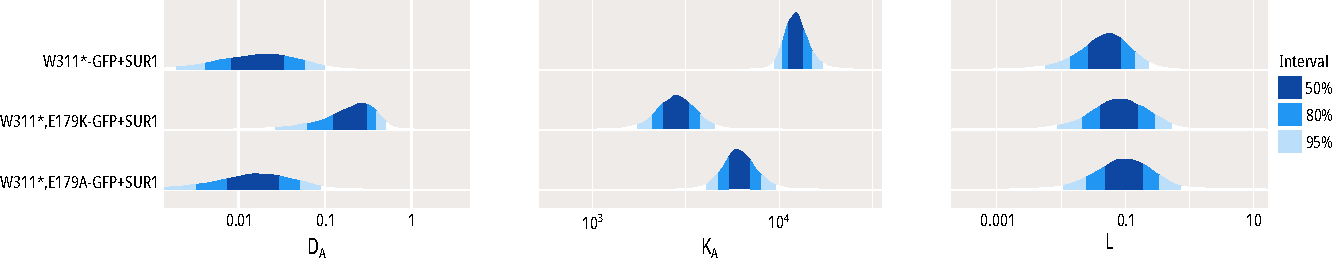
\includegraphics[width=\textwidth]{mwc_e179_2.pdf}
	\end{subfigure}
	\caption[E179 mutations affect gating and nucleotide binding]{
	\subref{ch5fig:mwc_e179_1} Current inhibition (orange) and fluorescence quenching (blue) from excised patches expressing W311*,E179A-GFP+SUR1 (left) or W311*,E179K-GFP+SUR1 (right).
	The smooth filled curves are the \SI{95}{\percent} intervals of the posterior probability distribution of fits to equations \ref{eq:mwc_binding} and \ref{eq:normalised_po}.
	Dashed curves are for comparison, and indicate the \SI{95}{\percent} intervals of the posterior probability distribution of fits to equations \ref{eq:mwc_binding} and \ref{eq:normalised_po} for the W311*-GFP+SUR1 data.
	\subref{ch5fig:mwc_e179_2} Posterior probability distributions for the estimated population $L$, $D$ and $K_A$ parameters from the fits in panel \subref{ch5fig:mwc_e179_1}.
	Each distribution is shaded with respect to its intervals.
	}\label{ch5fig:e179_2}
\end{figure}

\subsection{Mutations at K39 alter both inhibition and binding}

Residue K39 of Kir6.2 is located in the N-terminal region of Kir6.2, and is positioned between the inhibitory nucleotide binding site and the proposed PIP\textsubscript{2} binding site (Figure \ref{ch5fig:k39_loc}).
In previous studies, the mutation K39A has shown a small reduction in open probability \cite{cukras_role_2002}, and a small reduction in sensitivity to nucleotide inhibition \cite{cukras_role_2002, tucker_molecular_1998}.
These effects are somewhat contradictory, as mutations which reduce open probability tend also to increase sensitivity to nucleotide inhibition.
In each of the cryo-EM structures of K\ATP{}, the K39 side chain appears to coordinate the bound ATP molecule \cite{lee_molecular_2017, martin_anti-diabetic_2017, li_structure_2017, puljung_cryo-electron_2018-1}.
These structures are presumed to represent the closed state of the channel, and no PIP\textsubscript{2} bound structure of the channel has yet been solved.
However, molecular dynamics simulations using the ATP-bound structure as a starting point and introducing PIP\textsubscript{2} suggest that the K39 residue is able to contact both ligands (in press).
This suggests a potential role for K39 in the binding sites of both ATP and PIP\textsubscript{2}, which may explain the contradictory findings of open probability and nucleotide inhibition changes when the residue is mutated.

\begin{figure}[h]
	\centering
	\begin{subfigure}[t]{0.45\textwidth}
		\caption{}\label{ch5fig:k39_loc}
		\centering
		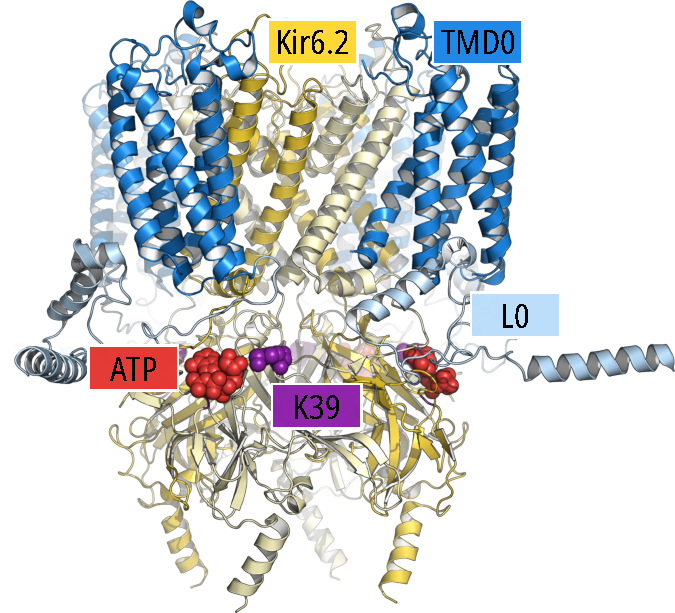
\includegraphics[width=\textwidth]{k39_1.pdf}
	\end{subfigure}
	\hfill
	\begin{subfigure}[t]{0.45\textwidth}
		\caption{}\label{ch5fig:k39_atp_popfits}
		\centering
		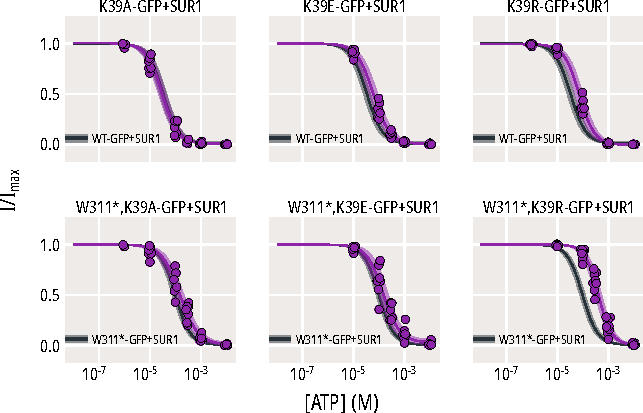
\includegraphics[width=\textwidth]{k39_2.pdf}
	\end{subfigure}
	\vfill
	\begin{subfigure}[t]{0.45\textwidth}
		\caption{}\label{ch5fig:k39_tnpatp_popfits_1}
		\centering
		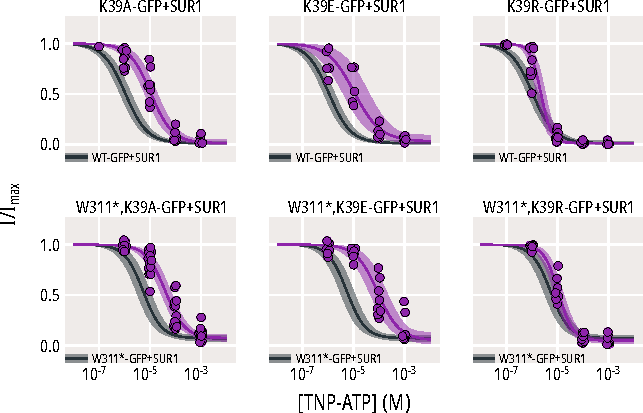
\includegraphics[width=\textwidth]{k39_3.pdf}
	\end{subfigure}
	\hfill
	\begin{subfigure}[t]{0.45\textwidth}
		\caption{}\label{ch5fig:k39_tnpatp_popfits_2}
		\centering
		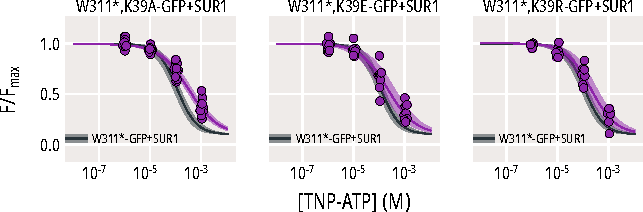
\includegraphics[width=\textwidth]{k39_4.pdf}
	\end{subfigure}
	\caption[Functional effects of K39 mutations]{
	\subref{ch5fig:k39_loc} Residue K39 is shown in purple in the cryo-EM structure of K\ATP{} (PDB \#6C3P).
	Adjacent subunits of Kir6.2 are shown in two different shades of yellow, TMD0 and L0 of SUR1 are shown in two different shades of blue.
	The core of SUR1 is not shown.
	Bound ATP is shown in red.
	\subref{ch5fig:k39_atp_popfits}, \subref{ch5fig:k39_tnpatp_popfits_1} Current inhibition of K39 mutants in the WT-GFP+SUR1 and W311*-GFP+SUR1 background by ATP (\subref{ch5fig:k39_atp_popfits}) or TNP-ATP (\subref{ch5fig:k39_tnpatp_popfits_1}).
	Each point represents an individual experiment.
	The smooth filled curves are the \SI{95}{\percent} intervals of the posterior probability distribution of fits to equation \ref{eq:hill} as described in the methods.
	\subref{ch5fig:k39_tnpatp_popfits_2} Fluorescence quenching of K39 mutants in the W311*-GFP+SUR1 background by TNP-ATP acquired simultaneously with the inhibition data in panel \subref{ch5fig:k39_tnpatp_popfits_1}.
	Each point represents an individual experiment.
	The smooth filled curves are the \SI{95}{\percent} intervals of the posterior probability distribution of fits to equation \ref{eq:hill} as described in the methods.
	}\label{ch5fig:k39_1}
\end{figure}

\begin{figure}[h]
	\centering
	\begin{subfigure}[t]{0.9\textwidth}
		\caption{}\label{ch5fig:k39_ec50_fits}
		\centering
		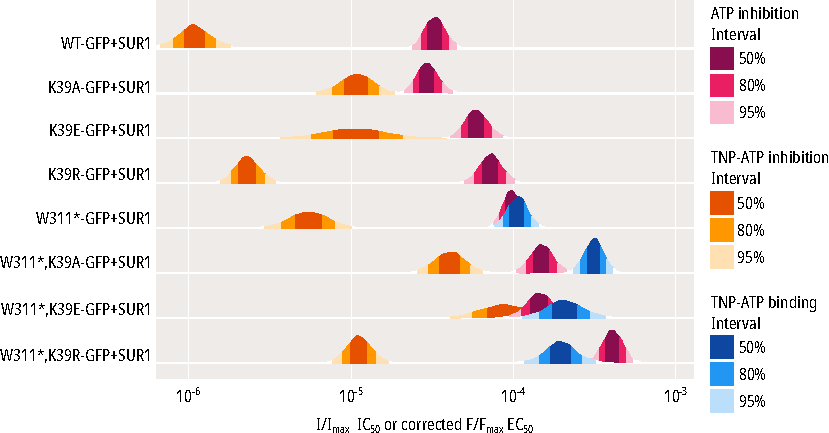
\includegraphics[width=\textwidth]{k39_5.pdf}
	\end{subfigure}
	\caption[K39 mutations $EC_{50}$ parameters]{
	\subref{ch5fig:k39_ec50_fits} Posterior probability distributions for the estimated population $IC_{50}$ or $EC_{50}$ values are shown in purple ($IC_{50}$ for ATP inhibition), orange ($IC_{50}$ for TNP-ATP inhibition), or blue ($EC_{50}$ for TNP-ATP binding).
	Each distribution is shaded with respect to its intervals.
	}\label{ch5fig:k39_1a}
\end{figure}

We tested three mutations at K39 (K39A, K39E, K39R) to examine the effects of changing the side chain characteristics on nucleotide binding and inhibition.
Mutation to E (opposite charge) or R (same charge) results in an increase in IC\textsubscript{50} for ATP inhibition for both WT and W311* backgrounds (Figure \ref{ch5fig:k39_atp_popfits}, \ref{ch5fig:k39_ec50_fits}).
We did not see an increase in the IC\textsubscript{50} for ATP inhibition when K39 was mutated to A (neutral) in either background (Figure \ref{ch5fig:k39_atp_popfits}, \ref{ch5fig:k39_ec50_fits}).
Inhibition by TNP-ATP displayed a different profile depending on the mutant residue (Figure \ref{ch5fig:k39_tnpatp_popfits_1}).
In both WT and W311* backgrounds, inhibition by TNP-ATP exhibited higher IC\textsubscript{50} values for K39A and K39E than we observed for K39R, which was not really distinguishable from K39 (\ref{ch5fig:k39_ec50_fits}).
Our docked conformation for TNP-ATP suggests that the TNP-moiety of the nucleotide may result in extra contacts with K39 compared to ATP, which may be the cause of the different sensitivity to inhibition between the two nucleotides when this residue is mutated.
Measurements of TNP-ATP binding showed increases in the EC\textsubscript{50} estimates for each of the three mutations (Figure \ref{ch5fig:k39_tnpatp_popfits_2}, \ref{ch5fig:k39_ec50_fits}).

Fits of the combined data to the MWC model gave parameter estimates for $K_A$ that decreased from K>R>E>A (Figure \ref{ch5fig:k39_2}).
In addition, mutation to an E or an A resulted in $D_A$ values closer to unity.
Interpretation of these parameters for the R and A mutations is frustrated by the differences in inhibition between TNP-ATP and ATP; we cannot be sure that these differences in binding and inhibition are due to the identity of the nucleotide rather than the identity of the residue.
However, the K39E mutation displayed similar inhibition for both TNP-ATP and ATP.
The increase in our estimate for $D_A$ when K39 is mutated to an A or an E, but not for R, may indicate a positive charge at the sidechain of this residue being important for transduction of nucleotide binding to the channel pore.

\begin{figure}[h]
	\centering
	\begin{subfigure}[t]{0.9\textwidth}
		\caption{}\label{ch5fig:mwc_k39_1}
		\centering
		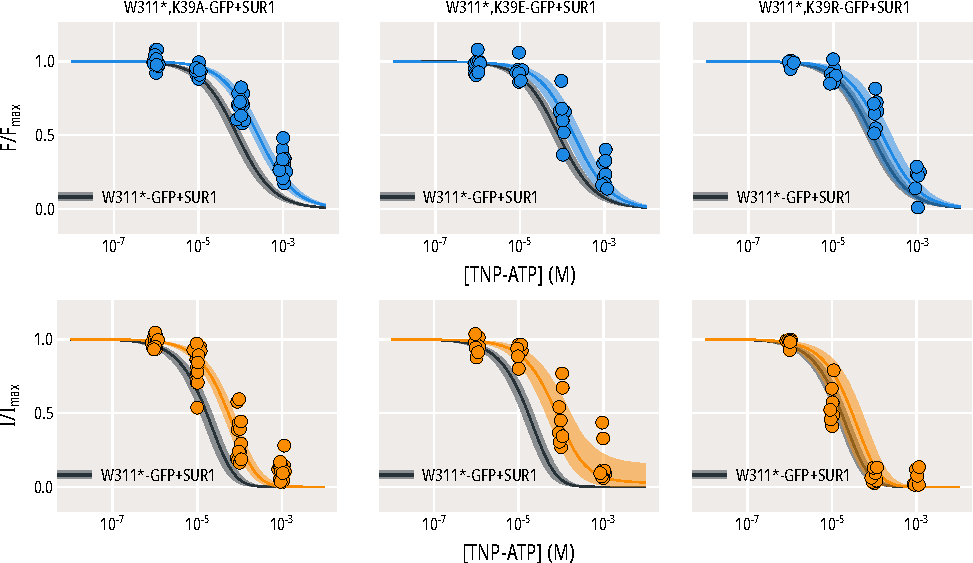
\includegraphics[width=\textwidth]{mwc_k39_1.pdf}
	\end{subfigure}
	\vfill
	\begin{subfigure}[t]{0.9\textwidth}
		\caption{}\label{ch5fig:mwc_k39_2}
		\centering
		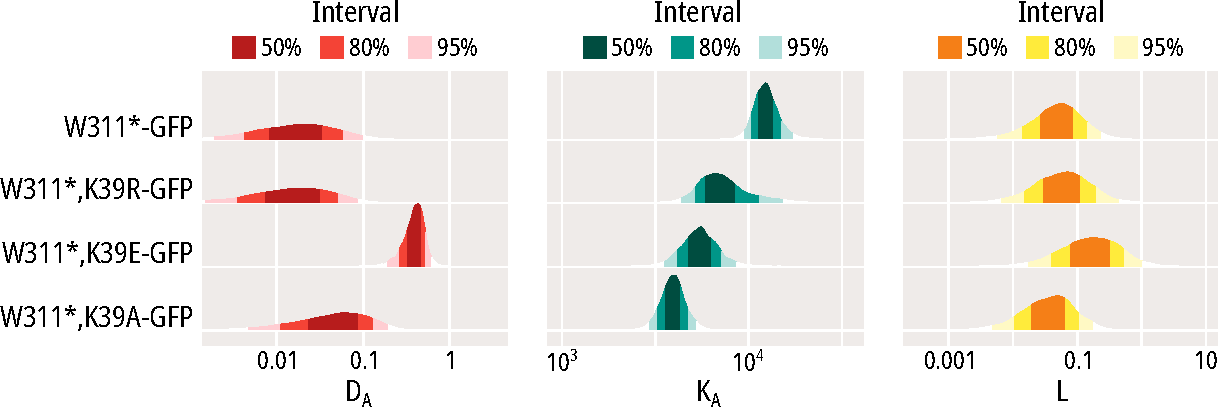
\includegraphics[width=\textwidth]{mwc_k39_2.pdf}
	\end{subfigure}
	\caption[K39 mutations affect gating and nucleotide binding]{
	\subref{ch5fig:mwc_k39_1} Current inhibition (orange) and fluorescence quenching (blue) from excised patches expressing W311*,K39A-GFP+SUR1 (left), W311*,K39E-GFP+SUR1 (middle), or W311*,K39R-GFP+SUR1 (right).
	The smooth filled curves are the \SI{95}{\percent} intervals of the posterior probability distribution of fits to equations \ref{eq:mwc_binding} and \ref{eq:normalised_po}.
	Dashed curves are for comparison, and indicate the \SI{95}{\percent} intervals of the posterior probability distribution of fits to equations \ref{eq:mwc_binding} and \ref{eq:normalised_po} for the W311*-GFP+SUR1 data.
	\subref{ch5fig:mwc_k39_2} Posterior probability distributions for the estimated population $L$, $D$ and $K_A$ parameters from the fits in panel \subref{ch5fig:mwc_k39_1}.
	Each distribution is shaded with respect to its intervals.
	}\label{ch5fig:k39_2}
\end{figure}

\section{Discussion}

Fitting a concerted MWC model to the combined datasets obtained by measuring TNP-ATP binding to Kir6.2 in combination with current inhibition allows us to distinguish between mutations which affect nucleotide binding, ligand-independent channel gating, and transduction of nucleotide binding to channel gating.
This is best demonstrated by our results for W311*,C166S-GFP+SUR1, which we propose not only increases the unliganded $P_O$ of the K\ATP{} channel as described many times previously (illustrated in this experiment by the increase in $L$ from the MWC fit), but also reduces the ability of TNP-ATP to induce channel closure ($D_A$ approaches unity).
Substitutions of C166 must therefore alter the structure of the channel such that in addition to the unliganded open state being more energetically favourable than in wild-type channels, nucleotides are no longer able to stabilise the closed state to the same extent as in wild type channels.

We can quantify this difference by calculating the energy contribution of nucleotide binding to the closed state of the two constructs at saturating concentrations of TNP-ATP, given by the formula $-RTln({D_A}^4)$ where $R$ is the gas constant and $T$ is the absolute temperature (assumed to be \SI{296}{\kelvin}).
The free energy TNP-ATP binding contributes to the closed state of W311*-GFP+SUR1 is \SIrange{23.0}{63.4}{\kilo\joule\per\Molar}, while the free energy TNP-ATP binding contributes to the closed state of W311*,C166S-GFP+SUR1 is only \SIrange{20.4}{-3.05}{\kilo\joule\per\Molar}.
However, as the transduction of binding is a combination of both the channel and the ligand, it is possible that TNP-ATP stabilises the closed state of the channel to a different extent than ATP.

Interpretation of our findings for substitutions at E179 and K39 of Kir6.2 are not as straightforward.
Mutations at these residues lead to a complex mixture of changes to both the microscopic binding affinity for TNP-ATP ($K_A$) and the transduction of nucleotide binding ($D_A$).
Given that E179 is predicted to form part of the PIP\textsubscript{2} binding site \cite{haider_identification_2007, pipatpolkai_evaluating_2020}, we might expect mutations at this location to alter the $P_O$ of channels in excised patches due to changes in the PIP\textsubscript{2} binding affinity.
\textcite{antcliff_functional_2005} found that mutation to asparagine increased the $P_O$ of K\ATP{} channels in excised patches, while \textcite{pipatpolkai_evaluating_2020} observed that mutation to a lysine caused a reduction in the IC\textsubscript{50} for neomycin inhibition of the channel.
Here, mutation to alanine or lysine did not result in a change in our estimate for $L$, which we would expect to see if there was a change in the $P_O$ of the channel resulting from altered OIP\textsubscript{2} affinity.
Instead, we observed changes in our estimates for $K_A$, the microscopic binding affinity for TNP-ATP, and $D_A$, the transduction of nucleotide binding to channel gating.

We believe there are two possible ways to interpret these findings.
The first is to accept the shift in $K_A$ at face value - a decrease in the apparent TNP-ATP binding affinity would suggest a role for residue E179 in forming the nucleotide binding pocket, and this function is abrogated by our mutations.
Despite the distance of the residue from the bound ATP, there could be interactions between E179 and the sidechains of residues which do form the pocket (e.g. R54), such that mutation of E179 leads to alterations in the binding pocket which reduce nucleotide binding affinity and therefore our estimate of $K_A$.
The additional effect on $D_A$ caused by mutating the residue to K suggests a dysregulation of the transduction of nucleotide binding to the channel pore, making nucleotides less selective for the closed state.

The second interpretation is possible due to the simplification of the role of PIP\textsubscript{2} in our MWC model as discussed in chapter \ref{ch:4}.
Briefly, if there is an additional allosteric interaction between nucleotide and PIP\textsubscript{2} binding to Kir6.2 which is separate to the channels open/closed state, then changes in $K_A$ may reflect alterations in the affinity for PIP\textsubscript{2} binding in addition to or instead of alterations in the affinity for nucleotide binding.
Thus, the decrease in $K_A$ upon mutation of E179 may reflect an increase in PIP\textsubscript{2} affinity and demonstrate the presence of local allostery between nucleotide and lipid.

Distinguishing between these two interpretations is difficult given our current evidence, and essentially depends on the weight you place on the assumptions of each, but should be possible with one or two further experiments.
Firstly, an increase in PIP\textsubscript{2} affinity should lead to an increase in channel open probability on excision (barring an effect on the relative preference of PIP\textsubscript{2} for the open state).
Our inability to accurately determine the open probability of the macroscopic experiments described so far could be supplemented by single channel analysis of the mutants to test this directly.
In addition, we could measure the affinity of PIP\textsubscript{2} directly in macroscopic patches.
Finally, to definitively test the existence of local allostery between the nucleotide and PIP\textsubscript{2} binding sites, we could introduce PIP\textsubscript{2} binding mutants into the C166S background.
C166S channels exhibit almost no nucleotide-dependent gating; i.e. nucleotide binding is uncoupled from gating of the channel pore.
Thus, any changes observed in nucleotide binding in the C166S background when PIP\textsubscript{2} affinity is changed would have to be due to a local allosteric interaction which does not involve the pore.

\begin{figure}[h]
	\centering
	\begin{subfigure}[t]{0.45\textwidth}
		\caption{}\label{ch5fig:k39_clash_atp}
		\centering
		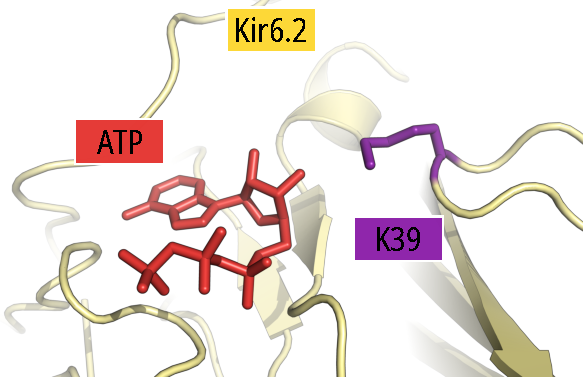
\includegraphics[width=\textwidth]{k39_clash_atp.pdf}
	\end{subfigure}
	\hfill
	\begin{subfigure}[t]{0.45\textwidth}
		\caption{}\label{ch5fig:k39_clash_tnpatp}
		\centering
		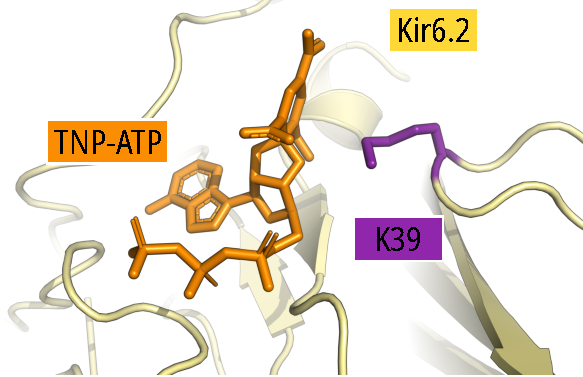
\includegraphics[width=\textwidth]{k39_clash_tnpatp.pdf}
	\end{subfigure}
	\caption[K39 is in close proximity to the TNP moiety of bound TNP-ATP]{
	\subref{ch5fig:k39_clash_atp}, \subref{ch5fig:k39_clash_tnpatp} Cryo-EM structure of ATP-bound K\ATP{} (PDB \# 6C3P) with residue K39 highlighted in purple.
	SHown as sticks is either the ATP molecule resolved in the cryo-EM structure (\subref{ch5fig:k39_clash_atp}, red) or a docked TNP-ATP molecule (\subref{ch5fig:k39_clash_tnpatp}, orange).
	}\label{ch5fig:k39_3}
\end{figure}

K39 is a residue which may be involved in both nucleotide and PIP\textsubscript{2} binding to Kir6.2, which may explain how mutation to an alanine at this residue appears to reduce both $P_O$ and sensitivity to nucleotide inhibiton \cite{cukras_role_2002, tucker_molecular_1998}.
We aimed to elucidate whether K39 was directly involved in nucleotide binding by making three different substitutions with different sidechain charges - alanine, lysine, or glutamic acid - and directly measuring TNP-ATP binding.
Unfortunately, we observed differences in the relative changes in inhibition by ATP and TNP-ATP in the three different constructs, such that the substitution which had the largest effect on ATP inhibition (K39R) had the smallest effect on TNP-ATP inhibition.
On examination of the cryo-EM structure of K\ATP{}, K39 is in close proximity to the ribose ring of bound ATP (Figure \ref{ch5fig:k39_clash_atp}).
The computational docking of TNP-ATP predicts that the TNP moiety will therefore be in close proximity of K39 (Figure \ref{ch5fig:k39_clash_tnpatp}).
Given this proximity, it is possible that there are extra contacts made between TNP-ATP and the K39 residue, which may go some way towards explaining the incresed sensitivity of inhibition of K\ATP{} to TNP-ATP.
It may also explain why we do not observe consistent relative changes in inhibition by ATP and TNP-ATP for different mutations of the residue.

However, given that substitutions of K39 decrease the sensitivity of K\ATP{} channels to ATP inhibition, and decrease both the sensitivity to TNP-ATP inhibition and the apparent TNP-ATP binding affinity, we can still conclude that K39 is involved in nucleotide binding to Kir6.2.
For TNP-ATP, this involvement manifests mostly as a reduction in the microscopic binding affinity ($K_A$), although substitution with a glutamic acid which has an oppositely-charged side chain also reduces the transduction of TNP-ATP binding to channel closure ($D_A$).
Despite the previously observed reduction in open probability for the K39A mutation \cite{cukras_role_2002, tucker_molecular_1998}, we did not observe any large changes in our estimates for $L$ for any of the mutations tested (Figure \ref{ch5fig:mwc_k39_2}).
There is some evidence to suggest that the identity of the amino acid at position 39 affects $P_O$, with K39A exhibiting an estimated $P_O$ range of \numrange{0.005}{0.15} compared to \numrange{0.017}{0.51} for K39E (Figure \ref{ch5fig:mwc_k39_2}); but given the uncertainty inherent in our data due to patch-to-patch differences in PIP\textsubscript{2} concentrations, run-down over the course of experiments, and having to normalise our data, we cannot confidently suggest there is an effect.